\documentclass[11pt]{article}

\usepackage[margin=1.1in]{geometry}
\usepackage{amsmath}
\usepackage{booktabs}
\usepackage{tikz}
\usepackage{microtype}

\title{Alloy\\[0.4em]
\large A machine-designed derivative-free optimizer,\\
and a full account of the search that found it}
\author{Peter Cotton}
\date{\today}

\begin{document}
\maketitle

\begin{abstract}
\noindent Alloy is a derivative-free optimizer for small evaluation budgets.
It was not written by a person: a language model generated it from a prompt
requiring an equal blend of Nelder--Mead, Differential Evolution, CMA-ES,
pattern search and simulated annealing, part by part
(Figure~\ref{fig:prompt} shows the prompt). On twenty-nine problems never
used in any selection step, Alloy has the best mean rank at every budget
from 60 to 480 evaluations and beats each of six competitors, including
CMA-ES, on 64\% to 77\% of 580 instances (sign-test $p < 10^{-10}$). It
ships in the humpday package. We describe the search construction that
produced it and report its failures candidly: the continuous search never
beat evaluating the obvious point, regenerations at the same recipe vary
severalfold, and a tuned generic template matched every selection score yet
collapsed out of sample. What survives is a recipe: one structured
generation step, validation on untouched problems, then distillation and
cheap tuning.
\end{abstract}

\section{The algorithm}

Alloy initialises with a Differential Evolution population and builds a
Nelder--Mead simplex from the best members. At each step it picks one of
four move generators with equal probability: a simplex
reflect-expand-contract step, a DE mutation with crossover, a Gaussian
perturbation with success-adapted diagonal covariance, or a Hooke--Jeeves
coordinate probe with a shrinking step.

Every candidate passes through a simulated-annealing acceptance gate with
geometric cooling. Stagnation triggers a reheat that rebuilds the simplex
around the incumbent.

Each ancestor is present as a mechanism, in the part of the algorithm it is
known for, at the frequency a recipe prescribed. That is because Alloy was
generated from a recipe, which the next section explains.

Its niche is small budgets, roughly 60 to 480 evaluations, on noisy or
irregular objectives. Nothing here claims it beats a tuned CMA-ES at fifty
thousand evaluations.

\section{How it was made}

Place $K$ established methods at the vertices of a simplex. A candidate is
a point $w = (w_1, \dots, w_K)$ with $w_k \ge 0$ and $\sum_k w_k = 1$: a
recipe saying how much of each ancestor a new program should contain
(Figure~\ref{fig:simplex}).

\begin{figure}[h]
\centering
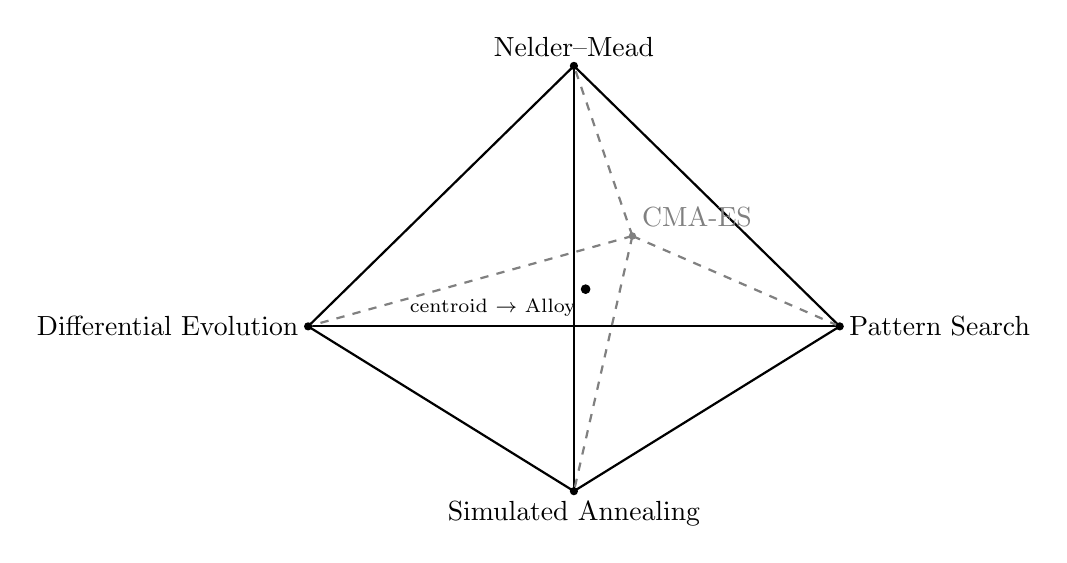
\begin{tikzpicture}[scale=1.35]
  \coordinate (NM) at (0, 2.0);
  \coordinate (DE) at (-2.5, -0.45);
  \coordinate (PS) at (2.5, -0.45);
  \coordinate (SA) at (0, -2.0);
  \coordinate (CMA) at (0.55, 0.4);
  % front edges of the 4-simplex
  \draw[thick] (NM) -- (DE) -- (SA) -- (PS) -- cycle;
  \draw[thick] (NM) -- (SA);
  \draw[thick] (DE) -- (PS);
  % edges receding to the rear vertex
  \draw[thick, dashed, gray] (CMA) -- (NM);
  \draw[thick, dashed, gray] (CMA) -- (DE);
  \draw[thick, dashed, gray] (CMA) -- (PS);
  \draw[thick, dashed, gray] (CMA) -- (SA);
  \fill (NM) circle (1.1pt) node[above] {Nelder--Mead};
  \fill (DE) circle (1.1pt) node[left] {Differential Evolution};
  \fill (PS) circle (1.1pt) node[right] {Pattern Search};
  \fill (SA) circle (1.1pt) node[below] {Simulated Annealing};
  \fill[gray] (CMA) circle (1.0pt) node[above right, gray] {CMA-ES};
  % the equal-weights centroid of all five vertices
  \coordinate (W) at (0.11, -0.1);
  \fill (W) circle (1.3pt);
  \node[below left] at (W) {\scriptsize centroid $\rightarrow$ Alloy};
\end{tikzpicture}
\caption{The five-vertex simplex drawn in perspective: a $4$-simplex has
ten edges, and the dashed ones recede to the rear vertex (CMA-ES). The
marked interior point is the equal-weights centroid, the recipe whose
prompt (Figure~\ref{fig:prompt}) produced Alloy.}
\label{fig:simplex}
\end{figure}

The example uses five classical methods as vertices:
Nelder--Mead~\cite{neldermead1965}, Differential
Evolution~\cite{stornprice1997}, CMA-ES~\cite{hansen2001}, pattern
search~\cite{hookejeeves1961}, and simulated
annealing~\cite{kirkpatrick1983}. The generator is a frontier language
model (\texttt{claude-opus-4-8}).

Every iterative optimizer has the same five parts: how it starts
(initialization), how it proposes the next candidate (move generation), how
it decides to keep or reject it (acceptance), how it adjusts step sizes
(adaptation), and when it restarts (restart).

Each vertex algorithm is famous for some parts and silent on others.
Differential evolution is a way of initialising and proposing moves;
simulated annealing is a way of accepting moves and restarting.

The heart of the map from recipe to program is an asymmetric instruction.
The heaviest vertex is the host and supplies the architecture; every other
vertex is a graft, and ``70\% A, 30\% B'' means ``A, but borrow an idea
from B'', not a chimera. What B's idea looks like inside A's architecture
is the model's decision.

The weights also set quantitative anchors. Each part is divided among the
vertices that have a mechanism for it, in proportion to their weights, and
the shares appear in the prompt as percentages: a vertex holding 25\% of
move generation means its move must be chosen a quarter of the time.

The coordinate therefore acts on two scales. Coarse changes act
semantically: they change who hosts, which ideas appear, and how
prominently. Fine changes, 20\% versus 15\% of a graft, move only the
percentages; at that scale the map is parametric.

Figure~\ref{fig:prompt} shows the actual prompt at the equal-weights
center: the point that produced Alloy. The prompt is a deterministic
function of the coordinate; the model decides how to implement each
mechanism and how to wire the parts together.

\begin{figure}[p]
\scriptsize
\begin{verbatim}
Build a black-box numerical optimizer by BLENDING base algorithms - but
blending is ASYMMETRIC, not a 50/50 average. The highest-weight method is
the HOST architecture; the others donate GRAFTED ideas in proportion to
their weight (a 30% method contributes a prominent borrowed mechanism; a 5%
method only a light inflection). '70% A, 30% B' means 'A, but borrow an
idea from B', not a chimera.

HOST architecture (20%): NelderMead - build the skeleton from this.
GRAFT into it: 20% DifferentialEvolution, 20% CMAEvolutionStrategy,
20% PatternSearch, 20% SimulatedAnnealing

Inspiration weights: NelderMead 20%, DifferentialEvolution 20%,
CMAEvolutionStrategy 20%, PatternSearch 20%, SimulatedAnnealing 20%

Per-slot guidance (host owns a slot unless a graft's weight dominates it):
  - initialization: DifferentialEvolution (100%): population +
    difference-vector mutation (rand/1, current-to-best/1) and crossover
  - move_generation: NelderMead (25%): downhill simplex: reflect/expand/
    contract/shrink a set of n+1 points; DifferentialEvolution (25%):
    population + difference-vector mutation and crossover;
    CMAEvolutionStrategy (25%): sample from a Gaussian whose covariance
    adapts to successful steps; PatternSearch (25%): Hooke-Jeeves
    coordinate moves with a step size that shrinks on failure
  - acceptance: SimulatedAnnealing (100%): accept uphill moves with
    probability exp(-dF/T); cool T over time
  - adaptation: NelderMead (33%); CMAEvolutionStrategy (33%);
    PatternSearch (33%)
  - restart: SimulatedAnnealing (100%)

Write connective glue as needed so the slots cooperate (e.g. the
acceptance rule gates the move-generation output; adaptation updates the
step/covariance used by move-generation). Favour a real, working blend
over a faithful copy of any single algorithm.

Write a single Python function with EXACTLY this signature and contract:

    def optimize(objective, n_trials, n_dim):
        """Minimise `objective` (a callable taking a list of n_dim floats
        in [0,1] and returning a float). Use AT MOST n_trials calls to
        objective. Return (best_value, best_point)."""

Hard rules:
  - Pure Python. You may `import math` and `import random` only.
  - Every candidate must be clipped into [0,1] before evaluation.
  - Count objective calls; never exceed n_trials.
  - No global state, no prints. Just the function.

Return ONLY a ```python code block containing the optimize function.
\end{verbatim}
\caption{The prompt that produced Alloy, at the equal-weights point
$w = (0.2, 0.2, 0.2, 0.2, 0.2)$, lightly line-wrapped for the page. Moving
$w$ changes the host, the graft proportions, and the per-slot shares, and
nothing else.}
\label{fig:prompt}
\end{figure}

Scoring the generated program on a benchmark assigns an objective value to
$w$, and the simplex maps to the unit cube by a standard bijection, so any
derivative-free optimizer can search it. Whether that search is worth
running is answered, mostly in the negative, in
Section~\ref{sec:negative}.

This idea sits between two traditions. Evolutionary and language-model
program search (genetic programming~\cite{koza1992}, evolutionary
art~\cite{sims1991}, FunSearch~\cite{funsearch2024},
AlphaEvolve~\cite{alphaevolve2025}, LLM variation
operators~\cite{lehman2022,meyerson2023}) explores a discrete artifact
space by sampling variations; algorithm configuration (algorithm
selection~\cite{rice1976}, hyper-heuristics~\cite{burke2013}) tunes the
constants of one frozen architecture. The simplex is continuous like the
second and architecturally open like the first.

\section{Evidence}

Candidates are scored on disguised versions of real-world objectives
(enzyme kinetics, wind-farm layout, battery dispatch, and others). A seeded
smooth bijection of the unit cube relocates each optimum, so a program
cannot succeed by memorisation.

The score is regret normalised against a panel of standard optimizers,
averaged over problems and seeds: 0 matches the best panel member
everywhere, 1 the worst. Selection used sixteen problems, three seeds, 120
evaluations per run.

\subsection{Selection}

Table~\ref{tab:warm} scores the five pure recipes and the equal-weights
centroid. Alloy, the centroid's program, wins at 0.087; the best pure
vertex, Nelder--Mead, scores 0.160.

\begin{table}[h]
\centering
\begin{tabular}{lc}
\toprule
recipe & regret \\
\midrule
centroid (equal fifths) $\rightarrow$ Alloy & 0.087 \\
pure Nelder--Mead & 0.160 \\
pure Simulated Annealing & 0.225 \\
pure Differential Evolution & 0.358 \\
pure Pattern Search & 0.477 \\
pure CMA-ES & 1.000 \\
\bottomrule
\end{tabular}
\caption{Panel-normalised regret (lower is better) of the program generated
at each recipe: sixteen disguised objectives, three seeds, 120 evaluations
per run.}
\label{tab:warm}
\end{table}

Structure mattered at generation time. Eight free-form attempts by the same
model, prompted simply for the strongest optimizer it could write, gave a
best of 0.141 and a median of 0.202 on the identical suite, against Alloy's
0.087.

\subsection{Validation on problems the search never saw}
\label{sec:heldout}

A selection winner can be a fluke, so the test that matters is out of
sample. Twenty-nine objectives, spanning 2 to 90 dimensions, were verified
against the full history of the benchmark library to have been used by no
selection step; each ran at budgets of 60, 120, 240 and 480 evaluations
with five seeds, 580 instances in all.

Alloy has the best mean rank and the most outright wins at every budget
against six competitors: Nelder--Mead, Differential Evolution, CMA-ES,
Nevergrad's CMA, a tuned 14-gene template, and the best free-form
generation. Pairwise it beats each of them on 64\% to 77\% of instances,
with sign-test $p$-values from $4\times10^{-11}$ down to
$1\times10^{-40}$.

Nor is it a lucky singleton. Adding the other strong selection-stage blends
gives Table~\ref{tab:untouched}: the blends hold the top four places at the
two smaller budgets, above every classical implementation, and the best of
them is statistically even with Alloy (48\% pairwise, $p = 0.29$).

\begin{table}[h]
\centering
\begin{tabular}{lcccc}
\toprule
 & \multicolumn{4}{c}{mean rank of 11 (lower is better)} \\
optimizer & 60 & 120 & 240 & 480 \\
\midrule
Alloy & 4.6 & 4.3 & 4.1 & 4.4 \\
warm4 blend (Patt 53, CMA 23) & 4.0 & 4.2 & 4.8 & 5.7 \\
rand14 blend (Patt 64, CMA 21) & 4.0 & 4.6 & 5.6 & 6.4 \\
14-gene template (evolved) & 5.8 & 5.6 & 5.3 & 5.4 \\
warm7 blend (Patt 92) & 5.0 & 5.1 & 5.9 & 7.4 \\
generated pure Nelder--Mead & 5.5 & 6.2 & 6.7 & 6.1 \\
Nevergrad CMA & 6.7 & 6.6 & 5.9 & 5.7 \\
Differential Evolution & 7.6 & 7.0 & 6.4 & 5.2 \\
CMA-ES & 7.7 & 7.1 & 6.3 & 5.7 \\
free-form best & 6.8 & 7.3 & 6.9 & 6.4 \\
Nelder--Mead & 7.8 & 7.8 & 7.7 & 7.1 \\
\bottomrule
\end{tabular}
\caption{Race on the 29 held-out problems, 580 instances per budget column,
rows ordered by mean rank across budgets. Blends dominate at small budgets;
Alloy is the most consistent.}
\label{tab:untouched}
\end{table}

The recipes genuinely differ out of sample. The nearly pure pattern-search
blend fades at 480 evaluations while Alloy stays first, so the coordinate
carries information, not just the generator.

A distilled twin performs identically. Rewriting Alloy's architecture as
one ordinary program with the mixing proportions as parameters, then tuning
those with twenty cheap evaluations, gives an optimizer statistically even
with Alloy on the held-out race (45\% pairwise, $p = 0.05$) with no
language model anywhere at run time.

\section{What did not work}
\label{sec:negative}

These negative results are half the point of this note, and each changed
what we believe.

The continuous search never earned its keep. The winning recipe was the
centroid, the one point anyone would evaluate first; twenty-five random
interior points, a warm-neighbourhood sweep, and a guided derivative-free
outer loop (best-of-twenty 0.270 versus 0.308 for random sampling) all
found nothing better. A second round with unequal vertices confirmed the
diagnosis: there the equal blend was mid-pack, and the best point was again
a vertex, so the centroid's win reflects a symmetric vertex set, not a
generally rich interior.

Generation is a lottery. Five draws at the centroid recipe scored 0.087,
0.249, 0.301, 0.320 and 1.000, and roughly one generation in seven fails to
compile. Alloy is the validated draw, not the expected one; the procedure
that works samples a few draws and keeps what validates.

The map has blind spots. The pure CMA-ES recipe never produced a working
program: correct covariance adaptation is too much to write in budgeted
pure Python, and its generations were degenerate.

In-sample scores mislead, reliably. A 14-gene parametric template tuned by
evolutionary search posted the best selection score of anything we ran
(0.244) and then collapsed to mean rank 7 of 13 on the held-out problems.
Free-form one-shots sit at the bottom of every held-out table despite
respectable selection scores. Only races on untouched problems told the
truth.

Cheap parametric search matches expensive semantic search per evaluation.
On identical coordinates, a hand-parameterized version of Alloy's
architecture scored 0.272 in-sample where fresh language-model generations
scored 0.308; per point, the model does not pay for itself. Its value was
the architecture, found once.

Thin automatic tuning earns nothing. With generated programs exposing
eight or nine constants, fourteen inner evaluations never beat the model's
own defaults; descents began to work only with fewer constants and more
evaluations.

\section{What survives}

Seen from global optimization, the two-level structure is classical. The
semantic move is the basin hop and the parametric tuning is the local
descent~\cite{wales1997}; done inside the loop it is memetic
search~\cite{moscato1989}; the simplex is a continuous relaxation of
architecture choice, as in differentiable architecture
search~\cite{liu2019darts}; and the sample-cluster-descend workflow is
SHGO's~\cite{endres2018}, with the basins living in the space of generated
programs rather than in $w$.

The theory of those methods says to compare basin floors, not landing
points, and it is right here too: single-draw comparisons understate the
semantic layer, and the descents that worked were the ones given few
dimensions and enough evaluations.

The recipe that survives every experiment in this note: generate a small
number of structured blends, validate the winner on problems the search
never touched, distill it to a parametric family, and tune cheaply from
then on. The language model is used a handful of times, early, and never
again.

Anchoring also survives. Every simplex point is a committee of mechanisms
that individually work, so even mediocre blends beat free-form generation
out of sample; and in an evolutionary loop, coordinate anchoring kept the
population about fifty percent more behaviorally diverse than free-form
iteration.

Nothing in the construction is specific to optimizers: it needs named
concepts the model knows, a decomposition of the artifact into parts, and a
measurable score. Whether other domains reproduce the pattern found here,
one excellent artifact and a mostly flat interior, is the open question.

The coordinates need not stay non-negative. A companion
note~\cite{outside2026} lets weights go negative, read as anti-inspirations
the program must steer away from; its best recipe won selection outright,
and an ablation then traced the entire win back inside the simplex, a
cautionary result recorded there in full.

\vspace{1em}
\noindent\emph{Availability.} Alloy ships in the humpday
package~\cite{humpday}, in Python and JavaScript. The search harness, the
run logs behind every number in this note, and every generated program are
in the same repository.

\begin{thebibliography}{9}

\bibitem{humpday} P.~Cotton.
HumpDay: recommendations and comparisons of derivative-free optimizers.
\texttt{https://humpday.microprediction.org}, 2026.

\bibitem{outside2026} P.~Cotton.
Thinking outside the simplex: signed compositions of optimization
algorithms.
Working paper, \texttt{https://humpday.microprediction.org/papers.html},
2026.

\bibitem{koza1992} J.~R. Koza.
\emph{Genetic Programming: On the Programming of Computers by Means of
Natural Selection}. MIT Press, 1992.

\bibitem{sims1991} K.~Sims.
Artificial evolution for computer graphics.
\emph{Computer Graphics (SIGGRAPH)}, 25(4):319--328, 1991.

\bibitem{funsearch2024} B.~Romera-Paredes et al.
Mathematical discoveries from program search with large language models.
\emph{Nature}, 625:468--475, 2024.

\bibitem{alphaevolve2025} A.~Novikov et al.
AlphaEvolve: a coding agent for scientific and algorithmic discovery.
Google DeepMind technical report, 2025.

\bibitem{lehman2022} J.~Lehman, J.~Gordon, S.~Jain, K.~Ndousse, C.~Yeh, and
K.~O. Stanley. Evolution through large models.
arXiv:2206.08896, 2022.

\bibitem{meyerson2023} E.~Meyerson, M.~J. Nelson, H.~Bradley, A.~Gaier,
A.~Moradi, A.~K. Hoover, and J.~Lehman.
Language model crossover: variation through few-shot prompting.
arXiv:2302.12170, 2023.

\bibitem{rice1976} J.~R. Rice.
The algorithm selection problem.
\emph{Advances in Computers}, 15:65--118, 1976.

\bibitem{neldermead1965} J.~A. Nelder and R.~Mead.
A simplex method for function minimization.
\emph{The Computer Journal}, 7(4):308--313, 1965.

\bibitem{stornprice1997} R.~Storn and K.~Price.
Differential evolution: a simple and efficient heuristic for global
optimization over continuous spaces.
\emph{Journal of Global Optimization}, 11:341--359, 1997.

\bibitem{hansen2001} N.~Hansen and A.~Ostermeier.
Completely derandomized self-adaptation in evolution strategies.
\emph{Evolutionary Computation}, 9(2):159--195, 2001.

\bibitem{hookejeeves1961} R.~Hooke and T.~A. Jeeves.
Direct search solution of numerical and statistical problems.
\emph{Journal of the ACM}, 8(2):212--229, 1961.

\bibitem{kirkpatrick1983} S.~Kirkpatrick, C.~D. Gelatt, and M.~P. Vecchi.
Optimization by simulated annealing.
\emph{Science}, 220(4598):671--680, 1983.

\bibitem{burke2013} E.~K. Burke, M.~Gendreau, M.~Hyde, G.~Kendall, G.~Ochoa,
E.~\"Ozcan, and R.~Qu.
Hyper-heuristics: a survey of the state of the art.
\emph{Journal of the Operational Research Society}, 64(12):1695--1724, 2013.

\bibitem{wales1997} D.~J. Wales and J.~P.~K. Doye.
Global optimization by basin-hopping and the lowest energy structures of
Lennard-Jones clusters.
\emph{Journal of Physical Chemistry A}, 101(28):5111--5116, 1997.

\bibitem{moscato1989} P.~Moscato.
On evolution, search, optimization, genetic algorithms and martial arts:
towards memetic algorithms.
Caltech C3P Report 826, 1989.

\bibitem{liu2019darts} H.~Liu, K.~Simonyan, and Y.~Yang.
DARTS: differentiable architecture search.
\emph{International Conference on Learning Representations}, 2019.

\bibitem{endres2018} S.~C. Endres, C.~Sandrock, and W.~W. Focke.
A simplicial homology algorithm for Lipschitz optimisation.
\emph{Journal of Global Optimization}, 72:181--217, 2018.

\end{thebibliography}

\end{document}
